\documentclass[12pt]{article}

\usepackage[utf8]{inputenc}
\usepackage{color,verbatim,Sweave,url,xargs,amsmath,hyperref,booktabs,longtable}
\usepackage[left=2cm,right=2cm,top=2cm,bottom=2cm]{geometry}
\usepackage{fancyhdr}
\usepackage{multicol}
\pagestyle{fancy}
\fancyhf{}

%% new commands
\makeatletter
\newcommand{\ID}[1]{\def\@ID{#1}}
\newcommand{\Date}[1]{\def\@Date{#1}}
\newcommand{\Titl}[1]{\def\@Titl{#1}}
\ID{00001}
\Date{YYYY-MM-DD}
\Titl{Title}

\Date{2019-09-04}
\ID{001}
\Titl{Frequency Tables, Dot Plots, Histograms}

\newcommand{\myID}{\@ID}
\newcommand{\myDate}{\@Date}
\newcommand{\myTitl}{\@Titl}
\makeatother

\lhead{\textsc{BHCC Mat-181}}
\rhead{\textsc{\myTitl}}

\usepackage{caption}
\captionsetup[figure]{labelformat=empty}

\usepackage{float}
\floatplacement{figure}{H}


%%% new environments
%\newenvironment{question}{\item \textbf{Problem}\newline}{\newpage}
%\newenvironment{solution}{\textbf{Solution}\newline}{\newpage}
%\newenvironment{answerlist}{\renewcommand{\labelenumi}{(\alph{enumi})}\begin{enumerate}}{\end{enumerate}}


%% compatibility with pandoc
\providecommand{\tightlist}{\setlength{\itemsep}{0pt}\setlength{\parskip}{0pt}}

%% fonts: Helvetica
\renewcommand{\sfdefault}{phv}
\IfFileExists{sfmath.sty}{
  \RequirePackage[helvet]{sfmath}
  \renewcommand{\rmdefault}{phv}
}{}

\newcommand{\extext}[1]{\textbf{\large #1}}
\newcommandx{\exmchoice}[9][2=-,3=-,4=-,5=-,6=-,7=-,8=-,9=-]{%
                \mbox{(a) \,\, \framebox[8mm]{\rule[-1mm]{0mm}{5mm} \hspace*{-1.6mm} \extext{#1}} \hspace*{2mm}}%
  \if #2- \else \mbox{(b) \,\, \framebox[8mm]{\rule[-1mm]{0mm}{5mm} \hspace*{-1.6mm} \extext{#2}} \hspace*{2mm}} \fi%
  \if #3- \else \mbox{(c) \,\, \framebox[8mm]{\rule[-1mm]{0mm}{5mm} \hspace*{-1.6mm} \extext{#3}} \hspace*{2mm}} \fi%
  \if #4- \else \mbox{(d) \,\, \framebox[8mm]{\rule[-1mm]{0mm}{5mm} \hspace*{-1.6mm} \extext{#4}} \hspace*{2mm}} \fi%
  \if #5- \else \mbox{(e) \,\, \framebox[8mm]{\rule[-1mm]{0mm}{5mm} \hspace*{-1.6mm} \extext{#5}} \hspace*{2mm}} \fi%
  \if #6- \else \mbox{(f) \,\, \framebox[8mm]{\rule[-1mm]{0mm}{5mm} \hspace*{-1.6mm} \extext{#6}} \hspace*{2mm}} \fi%
  \if #7- \else \mbox{(g) \,\, \framebox[8mm]{\rule[-1mm]{0mm}{5mm} \hspace*{-1.6mm} \extext{#7}} \hspace*{2mm}} \fi%
  \if #8- \else \mbox{(h) \,\, \framebox[8mm]{\rule[-1mm]{0mm}{5mm} \hspace*{-1.6mm} \extext{#8}} \hspace*{2mm}} \fi%
  \if #9- \else \mbox{(i) \,\, \framebox[8mm]{\rule[-1mm]{0mm}{5mm} \hspace*{-1.6mm} \extext{#9}} \hspace*{2mm}} \fi%
}
\newcommandx{\exclozechoice}[9][2=-,3=-,4=-,5=-,6=-,7=-,8=-,9=-]{\setcounter{enumiii}{1}%
                \mbox{\roman{enumiii}. \, \framebox[8mm]{\rule[-1mm]{0mm}{5mm} \hspace*{-1.6mm} \extext{#1}} \hspace*{2mm}\stepcounter{enumiii}}%
  \if #2- \else \mbox{\roman{enumiii}. \, \framebox[8mm]{\rule[-1mm]{0mm}{5mm} \hspace*{-1.6mm} \extext{#2}} \hspace*{2mm}\stepcounter{enumiii}} \fi%
  \if #3- \else \mbox{\roman{enumiii}. \, \framebox[8mm]{\rule[-1mm]{0mm}{5mm} \hspace*{-1.6mm} \extext{#3}} \hspace*{2mm}\stepcounter{enumiii}} \fi%
  \if #4- \else \mbox{\roman{enumiii}. \, \framebox[8mm]{\rule[-1mm]{0mm}{5mm} \hspace*{-1.6mm} \extext{#4}} \hspace*{2mm}\stepcounter{enumiii}} \fi%
  \if #5- \else \mbox{\roman{enumiii}. \, \framebox[8mm]{\rule[-1mm]{0mm}{5mm} \hspace*{-1.6mm} \extext{#5}} \hspace*{2mm}\stepcounter{enumiii}} \fi%
  \if #6- \else \mbox{\roman{enumiii}. \, \framebox[8mm]{\rule[-1mm]{0mm}{5mm} \hspace*{-1.6mm} \extext{#6}} \hspace*{2mm}\stepcounter{enumiii}} \fi%
  \if #7- \else \mbox{\roman{enumiii}. \, \framebox[8mm]{\rule[-1mm]{0mm}{5mm} \hspace*{-1.6mm} \extext{#7}} \hspace*{2mm}\stepcounter{enumiii}} \fi%
  \if #8- \else \mbox{\roman{enumiii}. \, \framebox[8mm]{\rule[-1mm]{0mm}{5mm} \hspace*{-1.6mm} \extext{#8}} \hspace*{2mm}\stepcounter{enumiii}} \fi%
  \if #9- \else \mbox{\roman{enumiii}. \, \framebox[8mm]{\rule[-1mm]{0mm}{5mm} \hspace*{-1.6mm} \extext{#9}} \hspace*{2mm}} \fi%
}
\newcommand{\exnum}[9]{%
  \mbox{\framebox[8mm]{\rule[-1mm]{0mm}{5mm} \hspace*{-1.6mm} \extext{#1}}}%
  \mbox{\framebox[8mm]{\rule[-1mm]{0mm}{5mm} \hspace*{-1.6mm} \extext{#2}}}%
  \mbox{\framebox[8mm]{\rule[-1mm]{0mm}{5mm} \hspace*{-1.6mm} \extext{#3}}}%
  \mbox{\framebox[8mm]{\rule[-1mm]{0mm}{5mm} \hspace*{-1.6mm} \extext{#4}}}%
  \mbox{\framebox[8mm]{\rule[-1mm]{0mm}{5mm} \hspace*{-1.6mm} \extext{#5}}}%
  \mbox{\framebox[8mm]{\rule[-1mm]{0mm}{5mm} \hspace*{-1.6mm} \extext{#6}}}%
  \mbox{ \makebox[3mm]{\rule[-1mm]{0mm}{5mm} \hspace*{-2mm} .}}%
  \mbox{\framebox[8mm]{\rule[-1mm]{0mm}{5mm} \hspace*{-1.6mm} \extext{#7}}}%
  \mbox{\framebox[8mm]{\rule[-1mm]{0mm}{5mm} \hspace*{-1.6mm} \extext{#8}}}%
  \mbox{\framebox[8mm]{\rule[-1mm]{0mm}{5mm} \hspace*{-1.6mm} \extext{#9}}}%
}
\newcommand{\exstring}[1]{%
  \mbox{\framebox[0.9\textwidth][l]{\rule[-1mm]{0mm}{5mm} \hspace*{-1.6mm} \extext{#1}} \hspace*{2mm}}%
}

%% new environments
\newenvironment{question}{\item \textbf{Problem:}\newline}{\newpage}
\newenvironment{solution}{\textbf{Solution:}}{\newpage}
\newenvironment{answerlist}{\renewcommand{\labelenumi}{(\alph{enumi})}\begin{enumerate}}{\end{enumerate}}


\begin{document}

\begin{enumerate}


\begin{question}
Please make a frequency table and a dot plot from the following
(unsorted) data.

\begin{longtable}[]{@{}rrrrr@{}}
\toprule
\endhead
17 & 17 & 16 & 15 & 13\tabularnewline
16 & 13 & 14 & 14 & 17\tabularnewline
18 & 15 & 18 & 17 & 11\tabularnewline
15 & 16 & 18 & 15 & 12\tabularnewline
\bottomrule
\end{longtable}
\end{question}

\begin{solution}
Make a frequency table.

\begin{longtable}[]{@{}rr@{}}
\toprule
value & frequency\tabularnewline
\midrule
\endhead
11 & 1\tabularnewline
12 & 1\tabularnewline
13 & 2\tabularnewline
14 & 2\tabularnewline
15 & 4\tabularnewline
16 & 3\tabularnewline
17 & 4\tabularnewline
18 & 3\tabularnewline
\bottomrule
\end{longtable}

Make the dot plot.

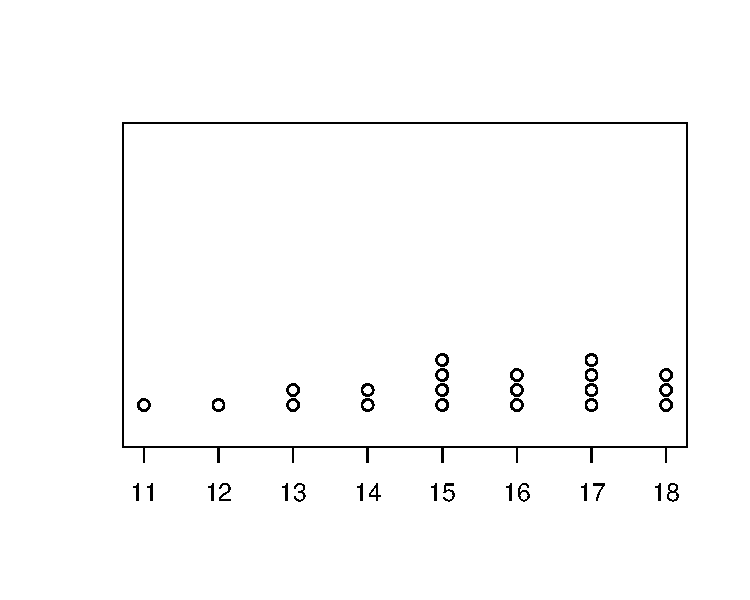
\includegraphics{hist-1.pdf}\\
\end{solution}



\begin{question}
Please make a frequency histogram from the following (unsorted)
continuous data by rounding to the nearest integer.

\begin{longtable}[]{@{}rrrrrr@{}}
\toprule
32.8201 & 27.7238 & 26.8074 & 29.1022 & 26.8669 & 31.1417\tabularnewline
27.2485 & 29.5684 & 32.2030 & 28.2653 & 27.0917 & 31.5793\tabularnewline
29.1215 & 27.6318 & 27.4419 & 29.8927 & 32.5300 & 26.7177\tabularnewline
30.3773 & 31.1362 & 30.5521 & 30.5156 & 31.8444 & 31.9692\tabularnewline
30.1981 & 31.9197 & 31.0182 & 31.5077 & 30.5075 & 28.5467\tabularnewline
\bottomrule
\end{longtable}
\end{question}

\begin{solution}
Make a frequency table.

\begin{longtable}[]{@{}rr@{}}
\toprule
value & frequency\tabularnewline
\midrule
\endhead
27 & 6\tabularnewline
28 & 3\tabularnewline
29 & 3\tabularnewline
30 & 4\tabularnewline
31 & 6\tabularnewline
32 & 6\tabularnewline
33 & 2\tabularnewline
\bottomrule
\end{longtable}

Make the histogram.

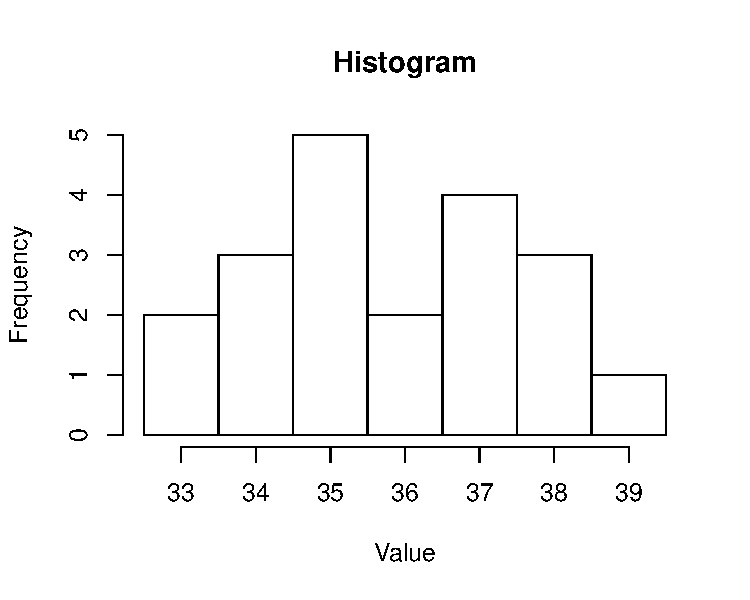
\includegraphics{barchart-1.pdf}\\
\end{solution}



\begin{question}
Please make a frequency table and a bar chart from the following
(unsorted) discrete data.

\begin{longtable}[]{@{}rrrrr@{}}
\toprule
\endhead
24 & 25 & 23 & 25 & 26\tabularnewline
22 & 24 & 24 & 24 & 24\tabularnewline
23 & 25 & 24 & 25 & 26\tabularnewline
25 & 23 & 26 & 25 & 23\tabularnewline
\bottomrule
\end{longtable}
\end{question}

\begin{solution}
Make a frequency table.

\begin{longtable}[]{@{}rr@{}}
\toprule
value & frequency\tabularnewline
\midrule
\endhead
22 & 1\tabularnewline
23 & 4\tabularnewline
24 & 6\tabularnewline
25 & 6\tabularnewline
26 & 3\tabularnewline
\bottomrule
\end{longtable}

Make the bar chart.

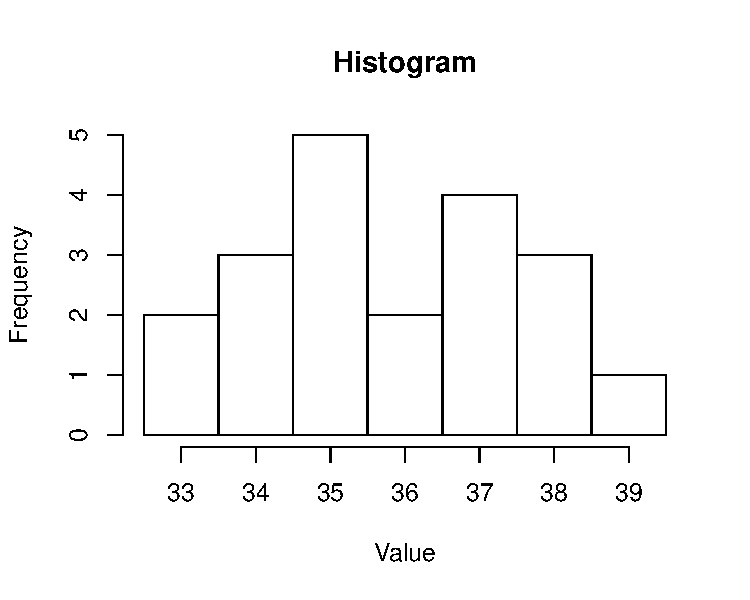
\includegraphics{barchart-1.pdf}\\
\end{solution}



\begin{question}
Please make a frequency table and a bar chart from the following
(unsorted) discrete data.

\begin{longtable}[]{@{}rrrrr@{}}
\toprule
\endhead
9 & 6 & 3 & 9 & 4\tabularnewline
6 & 8 & 6 & 9 & 5\tabularnewline
11 & 11 & 10 & 10 & 10\tabularnewline
9 & 7 & 10 & 10 & 6\tabularnewline
\bottomrule
\end{longtable}
\end{question}

\begin{solution}
Make a frequency table.

\begin{longtable}[]{@{}rr@{}}
\toprule
value & frequency\tabularnewline
\midrule
\endhead
3 & 1\tabularnewline
4 & 1\tabularnewline
5 & 1\tabularnewline
6 & 4\tabularnewline
7 & 1\tabularnewline
8 & 1\tabularnewline
9 & 4\tabularnewline
10 & 5\tabularnewline
11 & 2\tabularnewline
\bottomrule
\end{longtable}

Make the bar chart.

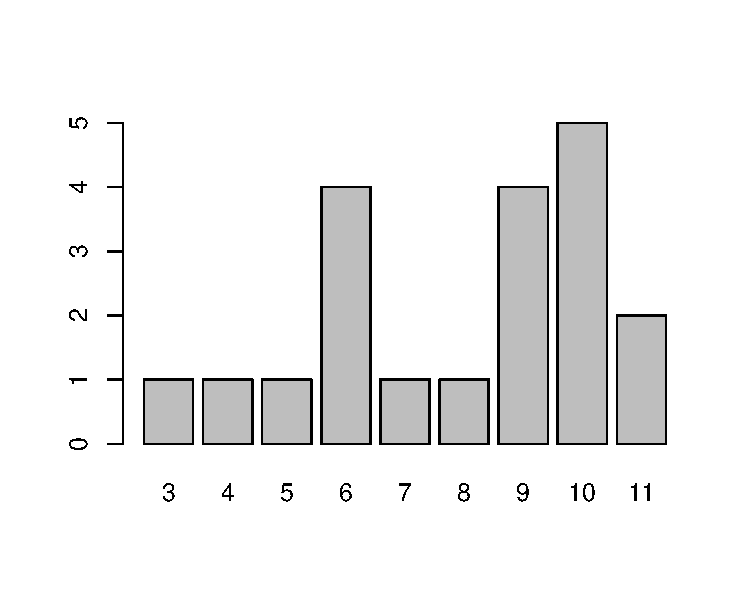
\includegraphics{barchart-1-3.pdf}\\
\end{solution}



\begin{question}
Please make a frequency table and a frequency histogram from the
following (unsorted) continuous data by rounding to the nearest integer.

\begin{longtable}[]{@{}rrrrrr@{}}
\toprule
\endhead
34.2282 & 33.4619 & 35.0504 & 36.5544 & 34.6125 & 32.7785\tabularnewline
35.2745 & 34.7295 & 35.8640 & 33.1210 & 34.7377 & 35.5176\tabularnewline
34.5648 & 33.8892 & 33.7858 & 33.4916 & 36.8922 & 33.6199\tabularnewline
37.3664 & 36.3487 & 36.5729 & 34.6641 & 33.0986 & 37.0611\tabularnewline
36.1932 & 35.8686 & 32.6269 & 37.3401 & 35.8037 & 32.3844\tabularnewline
\bottomrule
\end{longtable}
\end{question}

\begin{solution}
Make a frequency table.

\begin{longtable}[]{@{}rr@{}}
\toprule
bin & frequency\tabularnewline
\midrule
\endhead
32 & 1\tabularnewline
33 & 6\tabularnewline
34 & 4\tabularnewline
35 & 7\tabularnewline
36 & 6\tabularnewline
37 & 6\tabularnewline
\bottomrule
\end{longtable}

Make the histogram.

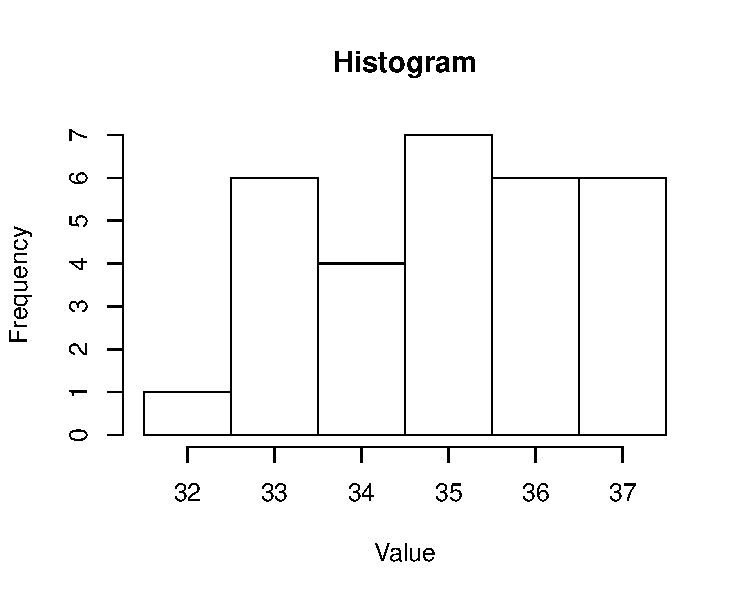
\includegraphics{barchart-1-4.pdf}\\
\end{solution}



\begin{question}
Please make a frequency table and a frequency histogram from the
following (unsorted) continuous data by rounding to the nearest integer.

\begin{longtable}[]{@{}rrrrrr@{}}
\toprule
\endhead
45.2712 & 44.1466 & 43.2676 & 43.8918 & 44.0346 & 45.8148\tabularnewline
47.1033 & 44.2204 & 44.3449 & 45.9275 & 44.4923 & 45.8552\tabularnewline
43.0629 & 45.1925 & 46.1901 & 42.4973 & 43.4716 & 46.6429\tabularnewline
43.5419 & 47.0171 & 43.4011 & 44.6069 & 47.0484 & 43.7841\tabularnewline
\bottomrule
\end{longtable}
\end{question}

\begin{solution}
Make a frequency table.

\begin{longtable}[]{@{}rr@{}}
\toprule
bin & frequency\tabularnewline
\midrule
\endhead
42 & 1\tabularnewline
43 & 4\tabularnewline
44 & 8\tabularnewline
45 & 3\tabularnewline
46 & 4\tabularnewline
47 & 4\tabularnewline
\bottomrule
\end{longtable}

Make the histogram.

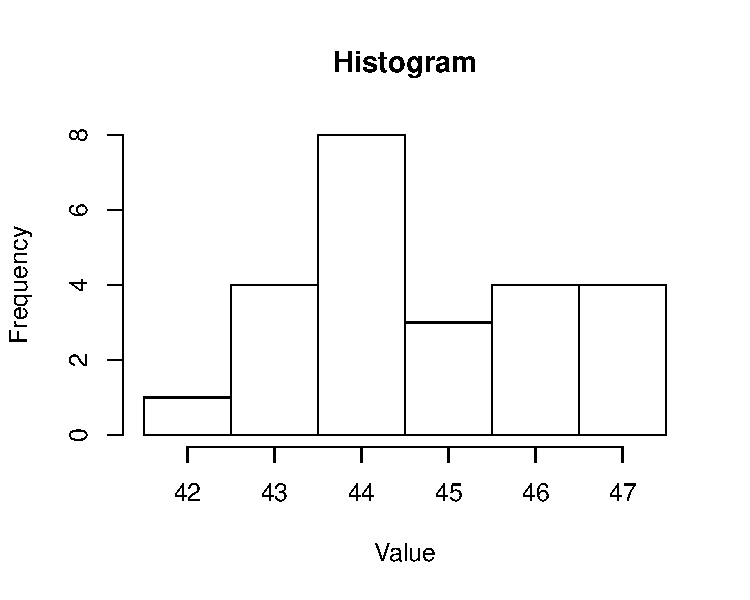
\includegraphics{barchart-1-5.pdf}\\
\end{solution}



\begin{question}
Please make a frequency table and a frequency histogram from the
following (sorted) continuous data by rounding to the nearest multiple
of 5.

\begin{longtable}[]{@{}rrrrr@{}}
\toprule
\endhead
39.0865 & 42.1185 & 43.0745 & 48.4095 & 50.4655\tabularnewline
53.6710 & 55.3400 & 57.4980 & 59.9800 & 60.3900\tabularnewline
60.6445 & 62.3565 & 62.8320 & 65.4455 & 65.9020\tabularnewline
66.1680 & 67.1330 & 67.5635 & 68.1090 & 68.9350\tabularnewline
69.1360 & 69.4095 & 69.7555 & 69.8470 & 70.7475\tabularnewline
70.9270 & 71.9800 & 72.1795 & 72.3365 & 74.1170\tabularnewline
\bottomrule
\end{longtable}
\end{question}

\begin{solution}
Make a frequency table.

\begin{longtable}[]{@{}rr@{}}
\toprule
bin & frequency\tabularnewline
\midrule
\endhead
40 & 2\tabularnewline
45 & 1\tabularnewline
50 & 2\tabularnewline
55 & 3\tabularnewline
60 & 4\tabularnewline
65 & 5\tabularnewline
70 & 12\tabularnewline
75 & 1\tabularnewline
\bottomrule
\end{longtable}

Make the histogram.

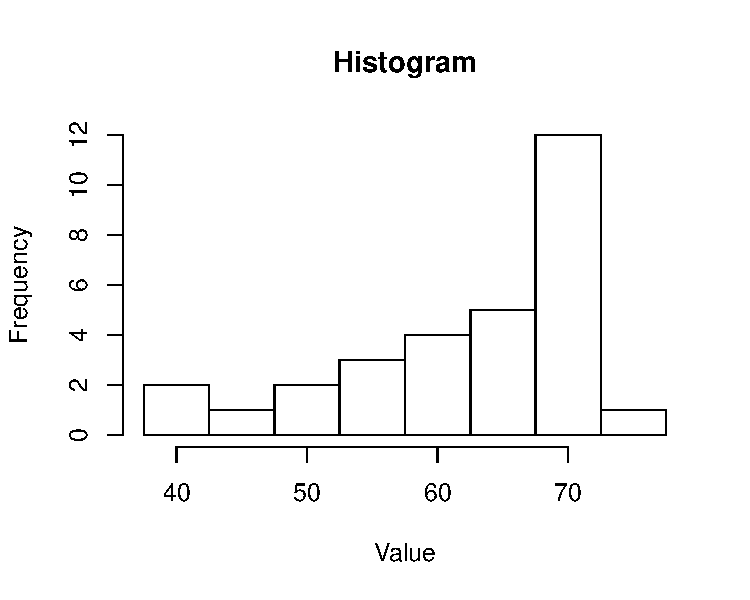
\includegraphics{barchart-1-6.pdf}\\
\end{solution}



\begin{question}
Please make a frequency table and a frequency histogram from the
following (sorted) continuous data by rounding to the nearest multiple
of 5.

\begin{longtable}[]{@{}rrrr@{}}
\toprule
\endhead
40.8440 & 41.0905 & 42.1430 & 43.2550\tabularnewline
43.5280 & 43.5585 & 44.2030 & 44.6110\tabularnewline
45.4230 & 46.4850 & 46.9060 & 47.1715\tabularnewline
47.1960 & 53.6380 & 58.5405 & 59.0435\tabularnewline
59.9515 & 60.0380 & 61.1855 & 64.4035\tabularnewline
64.5190 & 67.9745 & 69.2705 & 69.5665\tabularnewline
\bottomrule
\end{longtable}
\end{question}

\begin{solution}
Make a frequency table.

\begin{longtable}[]{@{}rr@{}}
\toprule
bin & frequency\tabularnewline
\midrule
\endhead
40 & 3\tabularnewline
45 & 10\tabularnewline
50 & 0\tabularnewline
55 & 1\tabularnewline
60 & 5\tabularnewline
65 & 2\tabularnewline
70 & 3\tabularnewline
\bottomrule
\end{longtable}

Make the histogram.

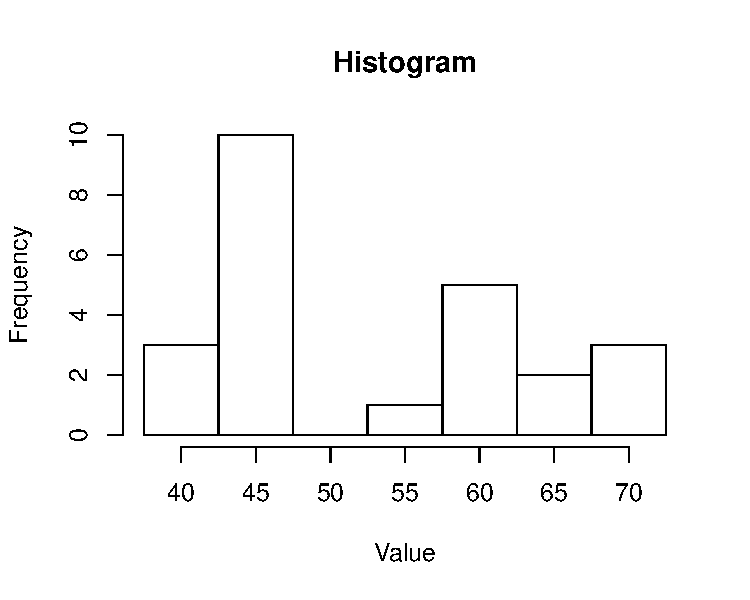
\includegraphics{barchart-1-7.pdf}\\
\end{solution}



\end{enumerate}


\end{document}
